\documentclass[12pt,a4paper,]{report}

\usepackage{perpage} %the perpage package
\MakePerPage{footnote} %the perpage package command

% ams
\usepackage{amssymb,amsmath}

\usepackage{ifxetex,ifluatex}
\usepackage{fixltx2e} % provides \textsubscript
\ifnum 0\ifxetex 1\fi\ifluatex 1\fi=0 % if pdftex
  \usepackage[T1]{fontenc}
  \usepackage[utf8]{inputenc}
\else % if luatex or xelatex
  \makeatletter
  \@ifpackageloaded{fontspec}{}{\usepackage{fontspec}}
  \makeatother
  \defaultfontfeatures{Ligatures=TeX,Scale=MatchLowercase}
  \makeatletter
  \@ifpackageloaded{soul}{
     \renewcommand\allcapsspacing[1]{{\addfontfeature{LetterSpace=15}#1}}
     \renewcommand\smallcapsspacing[1]{{\addfontfeature{LetterSpace=10}#1}}
   }{}
  \makeatother

% hard-coded fonts
\setmainfont[]{Roboto}
\setmonofont[]{Roboto}

\fi



% geometry
\usepackage[includehead, hmargin={3cm,3cm}, vmargin={2cm,3cm}, headsep=1.2cm, footskip=1.2cm]{geometry}

% figures placement
\usepackage{floatrow}
\floatsetup[figure]{capposition=top}
\floatplacement{figure}{H}

% headers
\usepackage{fancyhdr}
\renewcommand{\headruleskip}{10pt} %distance between headrule and header content
\renewcommand{\footnoterule}{\vfill\kern -3pt \hrule width 0.4\columnwidth \kern 2.6pt}

\pagestyle{fancy}
\fancyhead[R]{
\includegraphics[height=12pt]{logos/scholaLogoNew}}

\fancyhead[L]{
\includegraphics[height=25pt]{logos/eduzmena}}


% atypical captions above figures
\usepackage{caption}
\captionsetup{justification=raggedright,singlelinecheck=false,belowskip=0pt}

% graphix
\usepackage{graphicx}
\setkeys{Gin}{width=\linewidth,totalheight=\textheight,keepaspectratio}

% booktabs
\usepackage{booktabs}

% url
\usepackage{url}

% hyperref
\usepackage{hyperref}

% units.
\usepackage{units}

% use babel whatever engine is used
  \usepackage[main=czech]{babel}
\addto\captionsenglish{\renewcommand{\figurename}{Fig.}}
\addto\captionsczech{\renewcommand{\figurename}{Graf}}


% microtype for better kernign etc.
\RequirePackage[final,babel=true]{microtype}
\DeclareMicrotypeBabelHook
  {czech}
  {kerning=, spacing=}

\setcounter{secnumdepth}{-1} %??

% citations


% pandoc syntax highlighting

% longtable
\usepackage{longtable,booktabs}

% multiplecol
\usepackage{multicol}

% strikeout
\usepackage[normalem]{ulem}

% morefloats
\usepackage{morefloats}

% spacing
\usepackage{setspace}

% and or a in the list of authors according to the lang variable
\newcommand{\tr}[2]{\ifnum\pdfstrcmp{\languagename}{czech}=0 #1\else #2\fi}

% tightlist macro required by pandoc >= 1.14
\providecommand{\tightlist}{%
  \setlength{\itemsep}{0pt}\setlength{\parskip}{0pt}}


\begin{document}

\begin{titlepage}
    \begin{center}

    \onehalfspacing

      \vspace*{1cm}

      \begin{figure}
      \centering
            
\includegraphics[width=4cm]{logos/eduzmena}%
      \hspace{1.5cm}%
            
\includegraphics[width=5cm]{logos/scholaLogoNew3}%
      \end{figure}

      \vspace{1cm}

      \textbf{\huge Výsledky z~dotazníku pro ředitele}

      \vspace{.25cm}

      \textit{\Large }

      \vspace{1cm}

      \large

      9. března~2021

      \vspace{1cm}

      výzkumný tým SCHOLA EMPIRICA

      \vspace{.25cm}

            Magdaléna Klimešová\footnote{Korespondenční autor. Kontakt: \href{mailto:klimesova@scholaempirica.org}{\nolinkurl{klimesova@scholaempirica.org}}}, Jaromír Mazák, Jan Netík, Aleš Vomáčka, Martina Koutná \tr{a}{and}~Marek Havrda
      
      
      \vspace{1.5cm}

    \end{center}
\end{titlepage}


\thispagestyle{empty}
\section*{Anotace}
Zpráva seznamuje s~výsledky šetření mezi řediteli v~rámci projektu Eduzměna, u~kterých jsme mapovali situaci v~celé řadě oblastí.

Dotazník se týkal profesního vzdělávání, zkušeností s~vedením školy, hodnocení jejího klimatu a~vybraných procesů ve škole, jakož i~vlastního pedagogického působení a~celkové spokojenosti s~prací.

Zmíněné oblasti jsme mapovali pomocí online dotazníku, jehož sběr probíhal v~rozmezí \linebreak 26. května~2020~\nobreakdash--~24. února~2021.

V~první části naleznete krátký komentář k~interpretaci použitých grafů, poté se věnujeme rovnou tomu nejzajímavějšímu a~sice výsledkům, které jsou vždy členěny na Vaší a~ostatní školy, abyste si mohli stav u~Vás snadno porovnat s~průměrem ostatních zapojených škol. Informace o~respondentech, včetně počtu zapojených vyučujících a~škol, naleznete za samotnými výsledky. Zpráva obsahuje také přílohu s~detailním pohledem na otázky, které v~těle zprávy prezentujeme souhrnně v~tzv. škálách (viz dále).

Přejeme Vám zajímavé a~inspirativní čtení a~věříme, že zpráva poslouží k~dalšímu rozvoji Vaší školy a~školního prostředí.


{
\renewcommand*\contentsname{Obsah zprávy}
\setcounter{tocdepth}{1}
\tableofcontents
}

\hypertarget{jak-se-zpruxe1vou-pracovat}{%
\chapter{Jak se zprávou pracovat}\label{jak-se-zpruxe1vou-pracovat}}

Následující text členíme do částí reflektující sekce dotazníků, který ředitelky a~ředitelé vyplňovali. Maximum informací se snažíme prezentovat pokud možno v~kompaktní grafické podobě. Ve zprávě využíváme tři typy grafů:

\hypertarget{krabicovuxfd-graf}{%
\subsection{Krabicový graf}\label{krabicovuxfd-graf}}

Krabicový graf (pro ukázku a~popis viz graf č. \ref{fig:boxplotDesc}) přehledně zobrazuje typické hodnoty:

\begin{itemize}
\tightlist
\item
  silnější linka vyznačuje medián\footnote{Pokud bychom seřadili jednotlivé respondenty podle počtu bodů v~dané položce, pak medián označuje hodnotu \emph{právě uprostřed} takové řady. Pokud je ředitelů sudý počet, jde o~průměr prostřední dvojice.},
\item
  šedá, vyplněná část ohraničuje~50~\% prostředních hodnot kolem mediánu (tj. mezi~25. a~75.~percentilem, na obrázku uvedeno jako „IQR``),
\item
  horizontální úsečky pak poukazují na~1,5násobek tohoto rozpětí.
\item
  Hodnoty mimo zmíněné části (vyobrazeny jako malé puntíky\footnote{V~případě, že stejnou odlehlou hodnotu zaujímá více učitelů, je puntík tmavější.}) představují mimořádně odlehlá pozorování či extrémy (tvoří dohromady méně než~1 \% dat).
  Samotné hodnoty jsou na ose „x`` (horizontální osa) a~tato osa má vždy rozsah podle toho, kolik bodů je v~dané škále možné získat.
\end{itemize}

Samotné hodnoty jsou na ose „x`` (horizontální osa).

\begin{figure}
{\centering 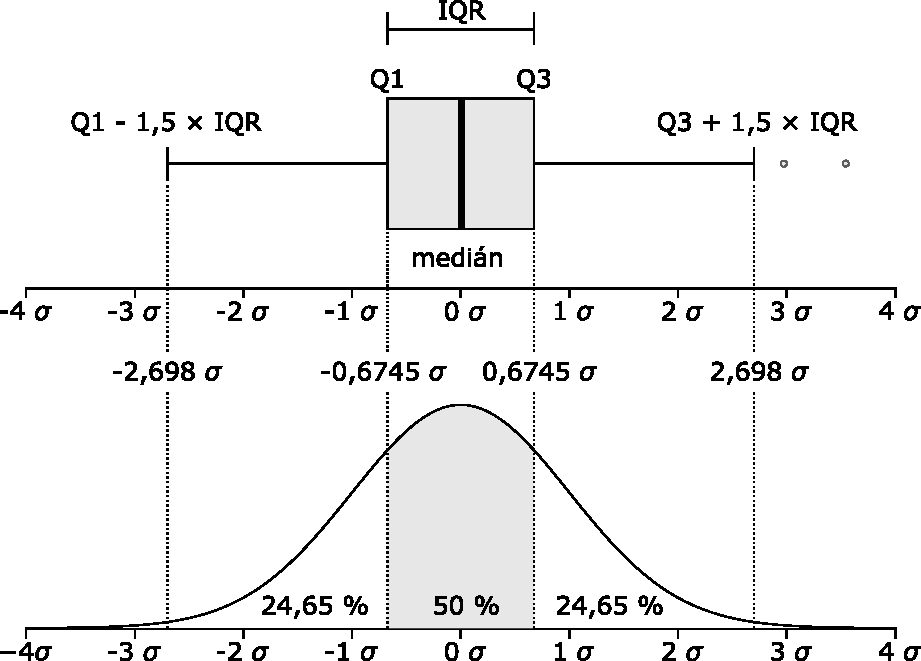
\includegraphics[width=0.75\textwidth]{figures/boxplot_description.pdf}}
\caption{Popis krabicového grafu ($\sigma$ značí směrodatnou odchylku, spodní část obrázku znázorňuje rozložení hodnot)}\label{fig:boxplotDesc}
\end{figure}

\hypertarget{skluxe1danuxfd-sloupcovuxfd-graf}{%
\subsection{Skládaný sloupcový graf}\label{skluxe1danuxfd-sloupcovuxfd-graf}}

Skládaný sloupcový graf vizualizuje podíl jednotlivých odpovědí (klíč k~barvám je vždy v~legendě) pro jednotlivé položky dotazníku. Čím větší plocha, tím větší má daná volba zastoupení. Osa „x`` je tedy vyjádřená v~procentech.

Na grafu č. \ref{fig:stackedBarPlot} můžete vidět příklad, kde je pro každou položku uveden jeden „řádek`` či pruh. Jednotlivé položky řadíme ve zprávě vždy podle součtu dvou nejvíce pozitivních kategorií (v případě grafu č. \ref{fig:stackedBarPlot} jde o~„Určitě ano`` a~„Spíše ano``). Pokud nemá položka dvojici „pólů`` (např. se týká časové frekvence) využíváme pouze spektra červené či modré (ta vždy označuje pozitivní, příznivější kategorie).

\begin{figure}

{\centering 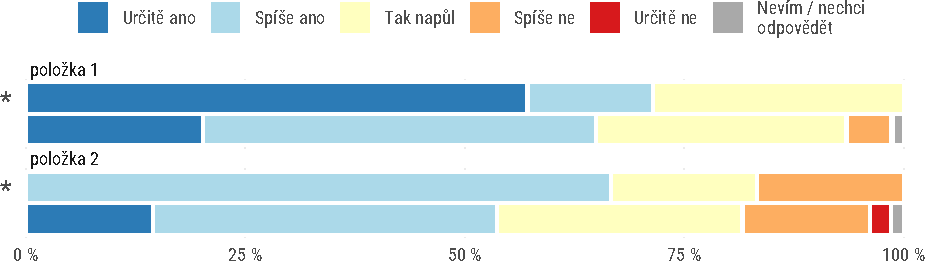
\includegraphics[width=\textwidth]{figs/stackedBarPlot-1} 

}

\caption{Ukázka skládaného sloupcového grafu}\label{fig:stackedBarPlot}
\end{figure}

\hypertarget{jednoduchuxfd-sloupcovuxfd-graf}{%
\subsection{Jednoduchý sloupcový graf}\label{jednoduchuxfd-sloupcovuxfd-graf}}

Graf níže pravděpodobně důvěrně znáte~-- jednotlivé odpovědi na jednu otázku jsou znázorněny šedivými sloupci, které reprezentují podíl dané odpovědi (uveden na konci sloupce).

\begin{figure}

{\centering 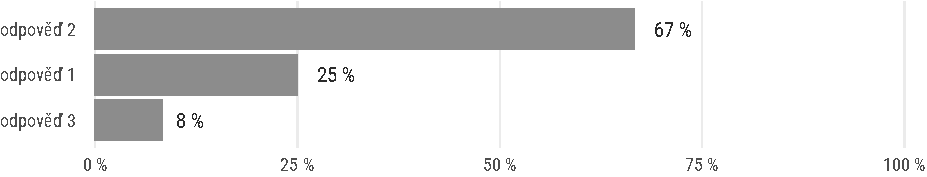
\includegraphics[width=\textwidth]{figs/unnamed-chunk-1-1} 

}

\caption{Ukázka sloupcového grafu}\label{fig:unnamed-chunk-1}
\end{figure}

\hypertarget{vuxfdsledky}{%
\chapter{Výsledky}\label{vuxfdsledky}}

\hypertarget{profesnuxed-vzdux11bluxe1vuxe1nuxed}{%
\section{Profesní vzdělávání}\label{profesnuxed-vzdux11bluxe1vuxe1nuxed}}

Následující grafy zachycují vybrané aspekty profesního vzdělávání ředitelů škol~-- účast na setkáních Místního akčního plánu rozvoje vzdělávání (MAP) a~jejich vnímanou užitečnost. Graf č. \ref{fig:profEduActivities} ukazuje konkrétní aktivity profesního vzdělávání. Poslední graf v~této sekci (č. \ref{fig:obst}) se týká pohledů ředitelů na vnímané překážky v~jejich účasti na profesním vzdělávání.

Více než polovina ředitelů uvádí, že se setkání MAP účastní pravidelně. Téměř pětina se však neúčastní vůbec.

\begin{figure}

{\centering 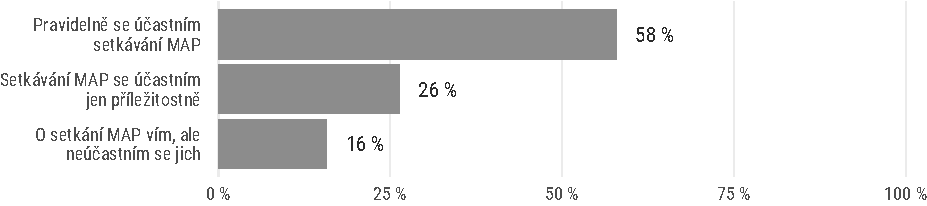
\includegraphics[width=\textwidth]{figs/map-1} 

}

\caption{Zapojení do Místního akčního plánu (MAP)}\label{fig:map}
\end{figure}

Z~těch, kdo se setkání alespoň někdy účastní, je skoro polovina považuje pro rozvoj školy za velmi užitečná a~polovina za spíše užitečná. Je ojedinělé, že by některý ředitel považoval setkání za neužitečná.

\begin{figure}

{\centering 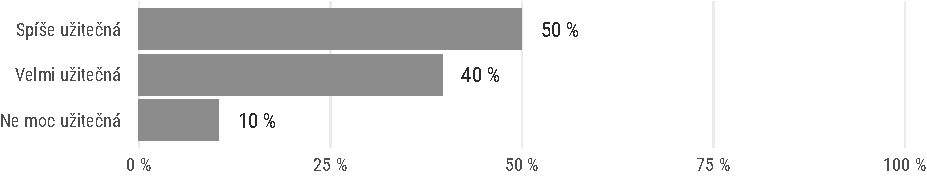
\includegraphics[width=\textwidth]{figs/unnamed-chunk-2-1} 

}

\caption{Užitečnost setkávání MAP pro rozvoj své školy}\label{fig:unnamed-chunk-2}
\end{figure}

Poměrně velká část ředitelů deklaruje, že se v~posledních dvanácti měsících účastnila nějaké aktivity profesního vzdělávání. Kromě kategorie „jiné``\footnote{Ředitelky a~ředitelé uváděli např. supervizní skupiny, individ. psychoterapii, seberozvoj, nácvik týmové spolupráce, letní čtenářskou školu, kurz zvládání krizových situací, diagnostiku psychologem práce a~organizace, metodické kurzy zaměřené na konkrétní metody, účast na výstavě učebních pomůcek, webináře zaměřené na formativní hodnocení atp.} je to vždy více než polovina ředitelů. Největší oblibě se těší četba odborné literatury.

\begin{figure}

{\centering 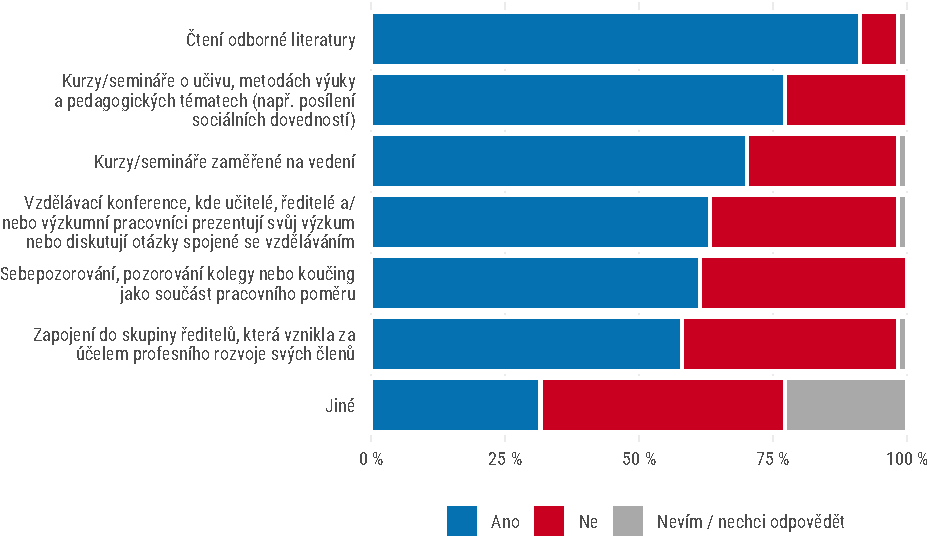
\includegraphics[width=\textwidth]{figs/profEduActivities-1} 

}

\caption{Aktivity v rámci profesního vzdělávání (za posledních 12 měsíců)}\label{fig:profEduActivities}
\end{figure}

Většina ředitelů neoznačuje žádnou z~překážek profesního vzdělávání uvedených níže za příliš silnou. Výjimkou je překážka vnímaná na straně zřizovatele, který profesní rozvoj podle necelých~20 \% respondentů dostatečně nepodporuje. Neopomenutelná část ředitelek a~ředitelů však na tuto položku odpověděla vyhýbavě, a~tak se lze domnnívat, že zastoupení souhlasných odpovědí bude ještě vyšší.

\begin{figure}

{\centering 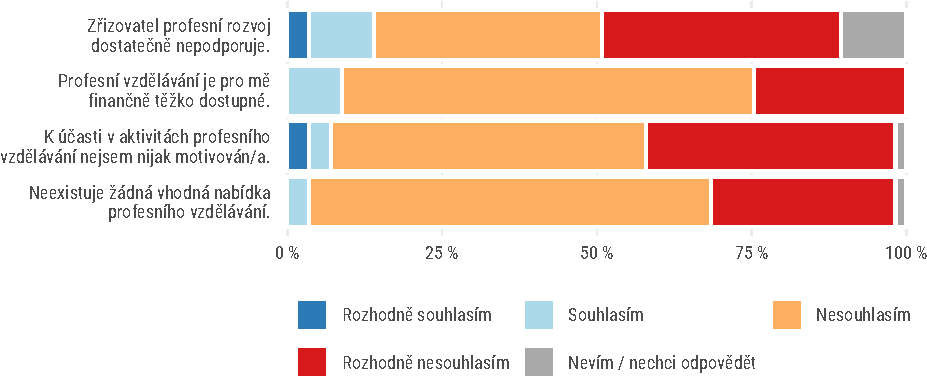
\includegraphics[width=\textwidth]{figs/obst-1} 

}

\caption{Vnímané překážky v účasti na profesním vzdělávání}\label{fig:obst}
\end{figure}

\newpage

\hypertarget{vedenuxed-ux161koly}{%
\section{Vedení školy}\label{vedenuxed-ux161koly}}

Tato sekce nabízí pohled na skladbu pracovní náplně ředitele školy.

Z~grafu č. \ref{fig:structure} je vidět, že u~některých aktivit existují mezi řediteli relativně velké rozdíly. Pro některé představuje administrativa do~20 \% pracovního času, ale pro jiné také~50 nebo i~více procent.

\begin{figure}

{\centering 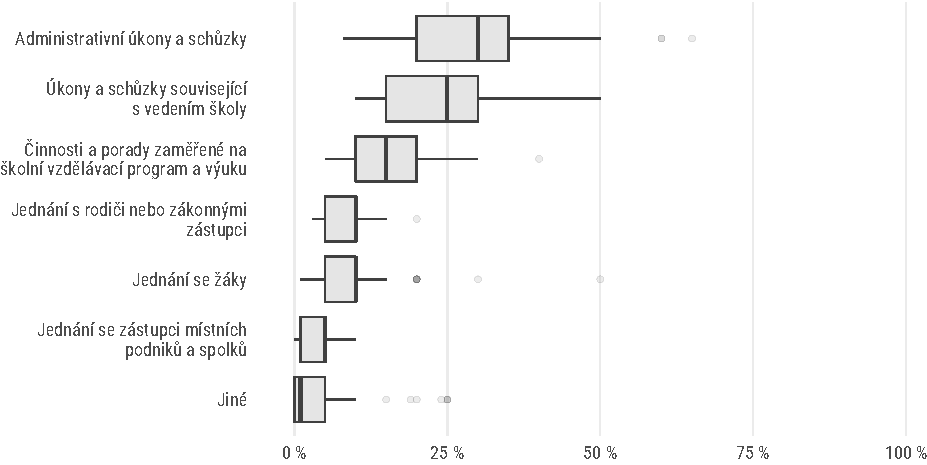
\includegraphics[width=\textwidth]{figs/structure-1} 

}

\caption{Zastoupení jednotlivých činností v práci ředitele za průměrný školní rok}\label{fig:structure}
\end{figure}

Z~hlediska sebehodnocení v~tom, jak jsou ředitelé proaktivní v~podpoře pedagogické práce učitelů, převažuje pozitivní sebehodnocení.

\begin{figure}

{\centering 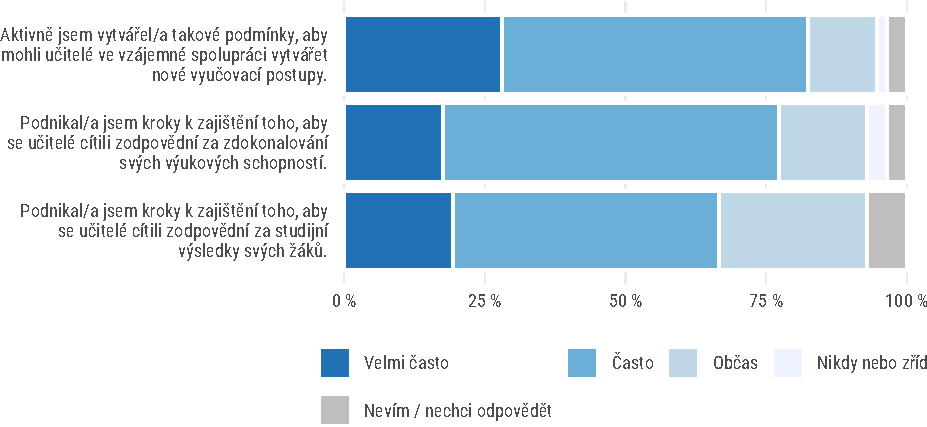
\includegraphics[width=\textwidth]{figs/proactive-1} 

}

\caption{Frekvence proaktivních kroků}\label{fig:proactive}
\end{figure}

\newpage

\hypertarget{klima-ux161koly}{%
\section{Klima školy}\label{klima-ux161koly}}

Sekce začíná shrnutím míry spolupráce s~různými aktéry, jako jsou rodiče či zákonní zástupci, pedagogicko-psychologické poradny, OSPOD aj. Následuje přehled vnímaných překážek v~poskytování kvalitní výuky a~graf shrnující činnosti kolem určitých patologických jevů či obecně problémového chování žáků.

\begin{figure}

{\centering 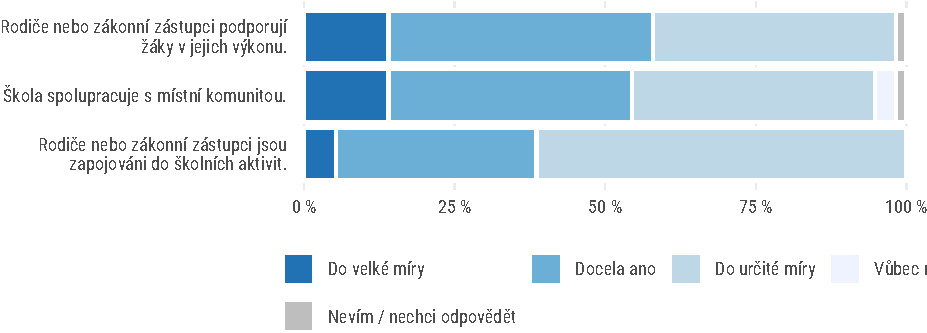
\includegraphics[width=\textwidth]{figs/coop-1} 

}

\caption{Spolupráce s rodiči a zapojení do místní komunity}\label{fig:coop}
\end{figure}

V~grafu č. \ref{fig:inst} kontrastuje poměrně velká míra spokojenosti spolupráce s~pedagogicko-psychologickými poradnami s~nezanedbatelnou částí ředitelů, kteří jsou naopak spíše nespokojeni se spoluprací s~OSPODem. Se středisky výchovné péča pak více jak čtvrtina škol spolupráci vůbec nenavázala nebo si nebyla odpovědí jistá.

\begin{figure}

{\centering 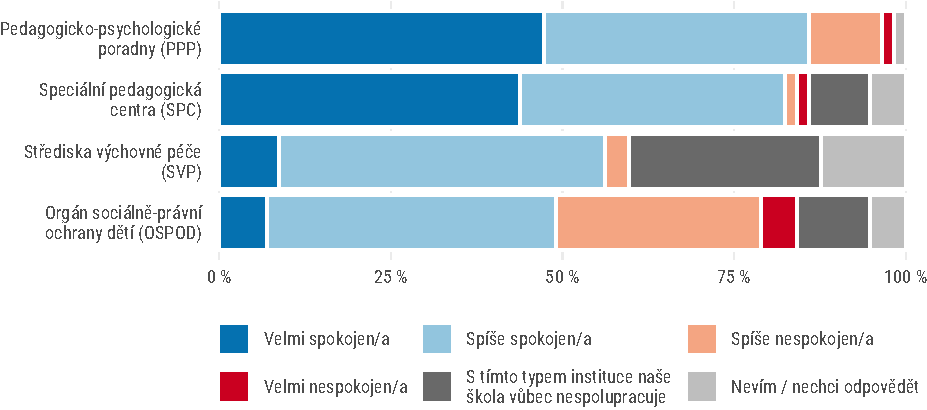
\includegraphics[width=\textwidth]{figs/inst-1} 

}

\caption{Spokojenost s podporou ze strany institucí}\label{fig:inst}
\end{figure}

Graf č. \ref{fig:obstacles} identifikuje, kde ředitelé nejčastěji vnímají překážky pro poskytování kvalitní výuky. Je seřazen podle součtu kategorií „do velké míry`` a~„docela ano``. Vede vnímaný nedostatek času na pedagogické vedení, kerý souvisí\footnote{A~to i~statisticky významně; Kendallovo \(\tau = 0,31; p = 0,004\).} s~podílem administrativních úkonů a~schůzek.

\begin{figure}

{\centering 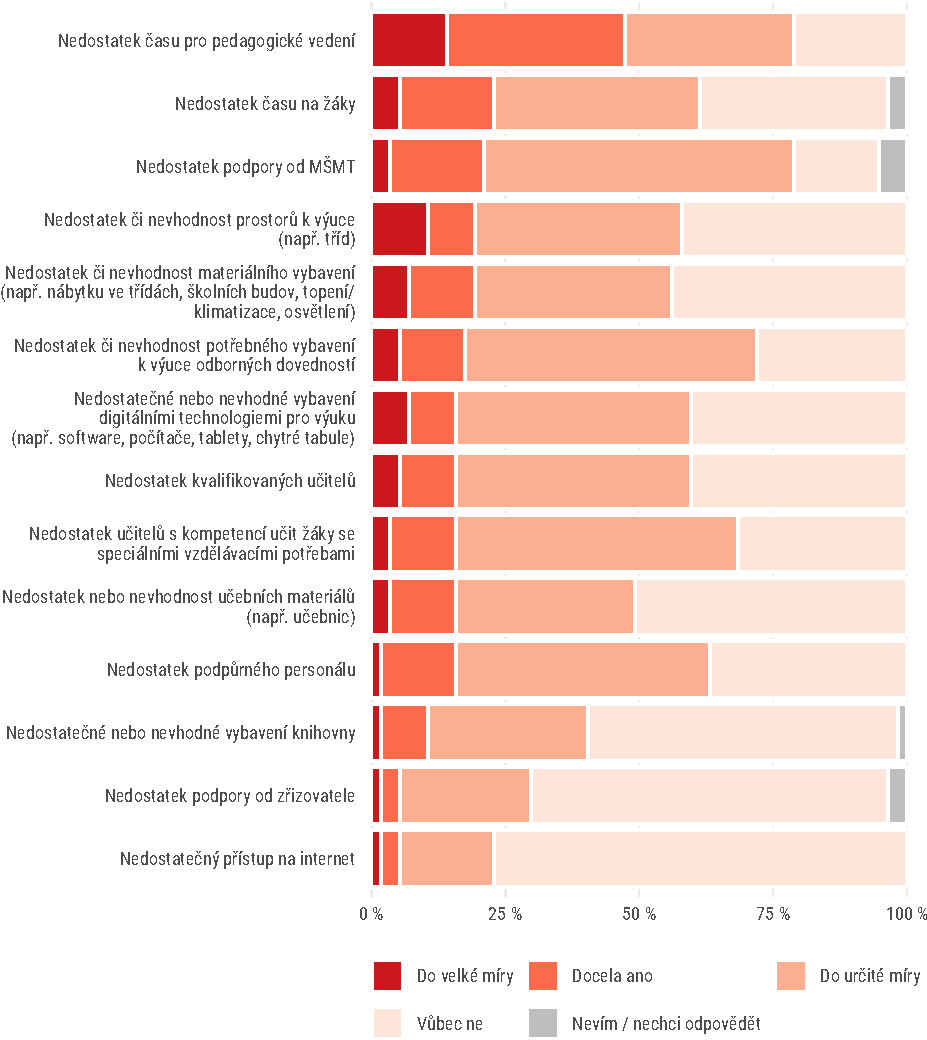
\includegraphics[width=\textwidth]{figs/obstacles-1} 

}

\caption{Překážky v poskytování kvalitní výuky}\label{fig:obstacles}
\end{figure}

U~nežádoucího chování, které musí ředitelé řešit, vystupují do popředí především šikana (včetně možné kyberšikany a~napadání učitelů) a~vandalstí a~krádeže. Fyzické násilí mezi žáky a~užívání drog je naopak méně časté.

\begin{figure}

{\centering 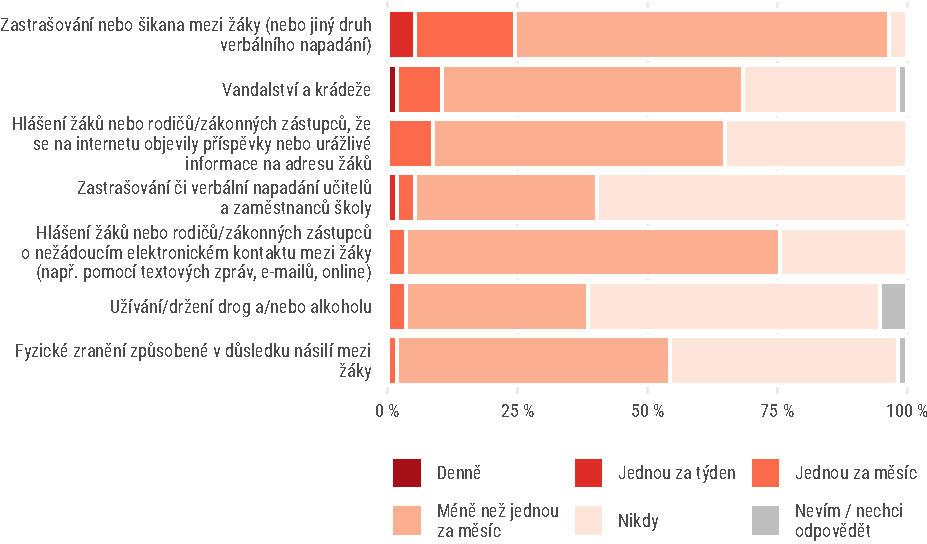
\includegraphics[width=\textwidth]{figs/delinq-1} 

}

\caption{Nežádoucí chování žáků}\label{fig:delinq}
\end{figure}

\hypertarget{zaux161kolovuxe1nuxed-a-mentorovuxe1nuxed}{%
\section{\texorpdfstring{Zaškolování a~mentorování}{Zaškolování amentorování}}\label{zaux161kolovuxe1nuxed-a-mentorovuxe1nuxed}}

Sekce shrnuje dostupnost neformálních i~formálních zaškolovacích aktivit, resp. programů a~jejich konkrétnější podobu, případně využívané nástroje či instituty.

Na více než polovině škol neexistuje pro nové učitele formální zaškolovací program.

\begin{figure}

{\centering 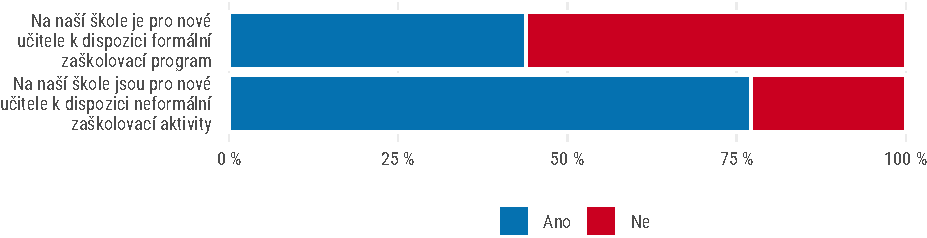
\includegraphics[width=\textwidth]{figs/unnamed-chunk-3-1} 

}

\caption{Dostupnost zaškolovacích aktivit}\label{fig:unnamed-chunk-3}
\end{figure}

Graf č. \ref{fig:activities} ukazuje podíl škol, na kterých jsou pro začínající učitele k~dispozici vybrané zaškolovací nástroje či aktivity. Zahrnuty jsou tedy jen školy, které alespoň na jednu z~předchozích dvou otázek odpověděli kladně.

\begin{figure}

{\centering 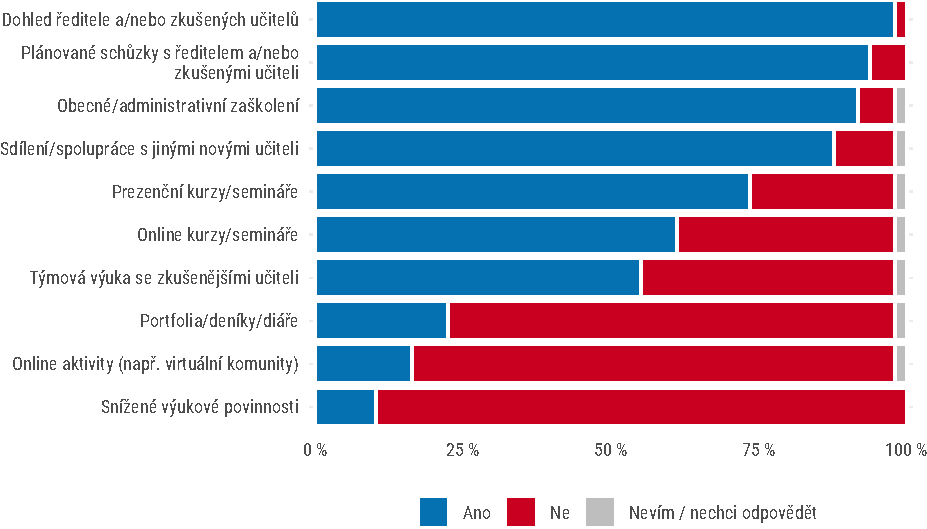
\includegraphics[width=\textwidth]{figs/activities-1} 

}

\caption{Nástroje a činnosti využívané k zaškolování nových učitelů}\label{fig:activities}
\end{figure}

\newpage

\hypertarget{vlastnuxed-pedagogickuxe9-pux16fsobenuxed}{%
\section{Vlastní pedagogické působení}\label{vlastnuxed-pedagogickuxe9-pux16fsobenuxed}}

Na pedagogické činnosti se aktivně podílí~56~(98,2 \%) ředitelů. Graf níže ukazuje, jakým způsobem:

\begin{figure}

{\centering 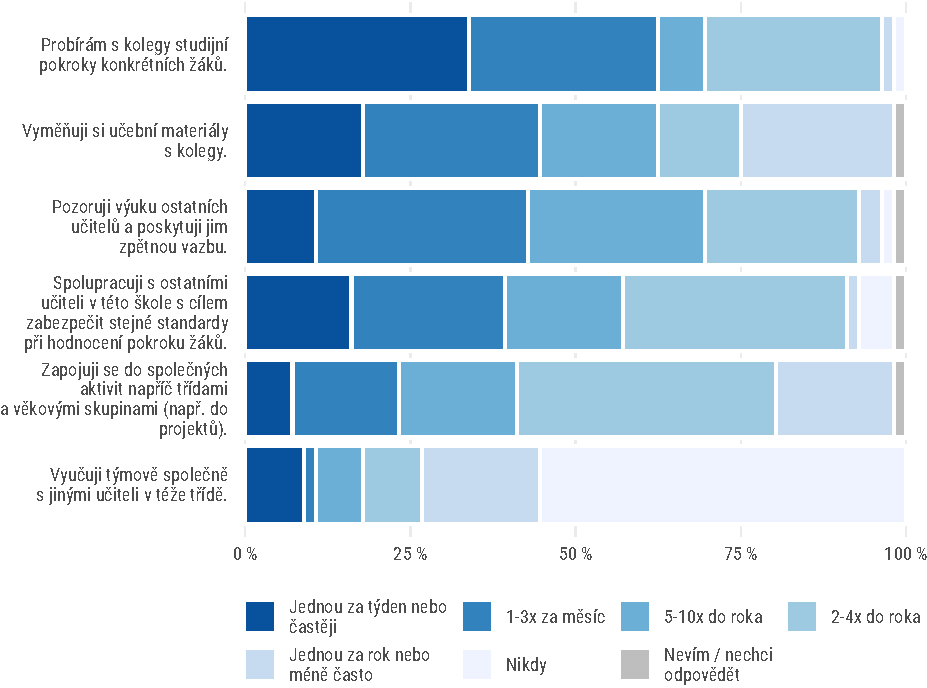
\includegraphics[width=\textwidth]{figs/teachPartic-1} 

}

\caption{Zapojení ředitelů do výuky}\label{fig:teachPartic}
\end{figure}

\hypertarget{spokojenost-s-pracuxed}{%
\section{\texorpdfstring{Spokojenost s~prací}{Spokojenost sprací}}\label{spokojenost-s-pracuxed}}

V~poslední sekci se věnujeme spokojenosti ředitele s~prací. Graf č. \ref{fig:motiv} ukazuje, kolik let by ředitelé ještě chtěli setrvat ve své pozici.

\begin{figure}

{\centering 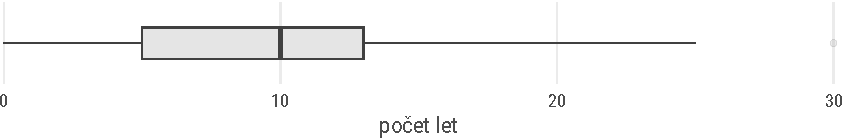
\includegraphics[width=\textwidth]{figs/motiv-1} 

}

\caption{Počet let, po který jsou ředitelé ochotni setrvat na své současné pracovní pozici}\label{fig:motiv}
\end{figure}

Potvrzuje se, co se často ozývalo již z~mapování potřeb, a~sice že mezi největší zdroje stresu pro ředitele patří administrativní zátěž a~také konkrétně nutnost vycházet vstříc měnícím se požadavkům správních orgánů. Možná překvapivě poměrně malým zdrojem stresu jsou aspekty týkající se udržování disciplíny. Také stojí za povšimnutí, že inkluze, resp. vycházení vstříc potřebám žáků se speciálními potřebami je výraznějším problémem jen v~menšině škol.

\begin{figure}

{\centering 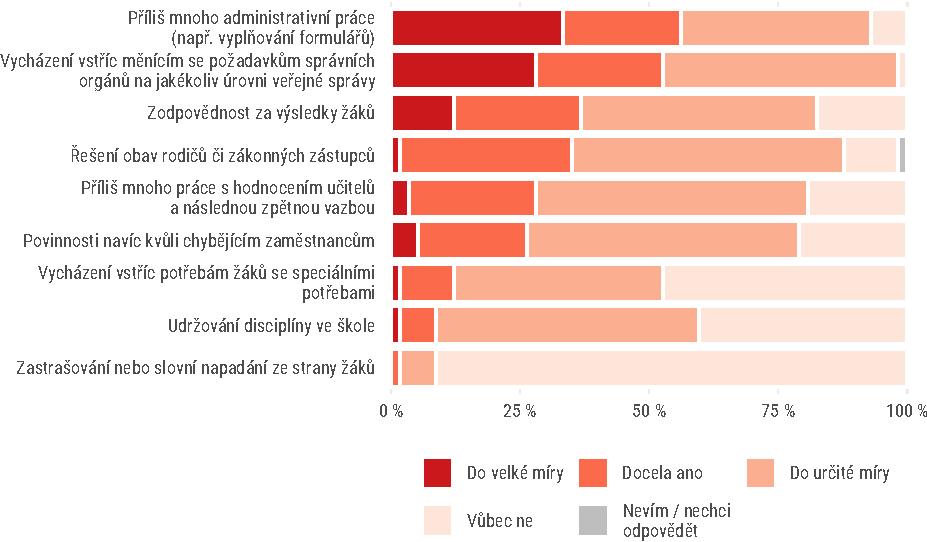
\includegraphics[width=\textwidth]{figs/stress-1} 

}

\caption{Vnímané zdroje pracovního stresu}\label{fig:stress}
\end{figure}

Dobrou zprávou je, že ředitelky a~ředitele celkově jejich práce těší. Svého rozhodnutí stát se ředitelem nelitují (pozor, v~grafu níže je u~této položky žádoucí \emph{záporná} odpověď).

\begin{figure}

{\centering 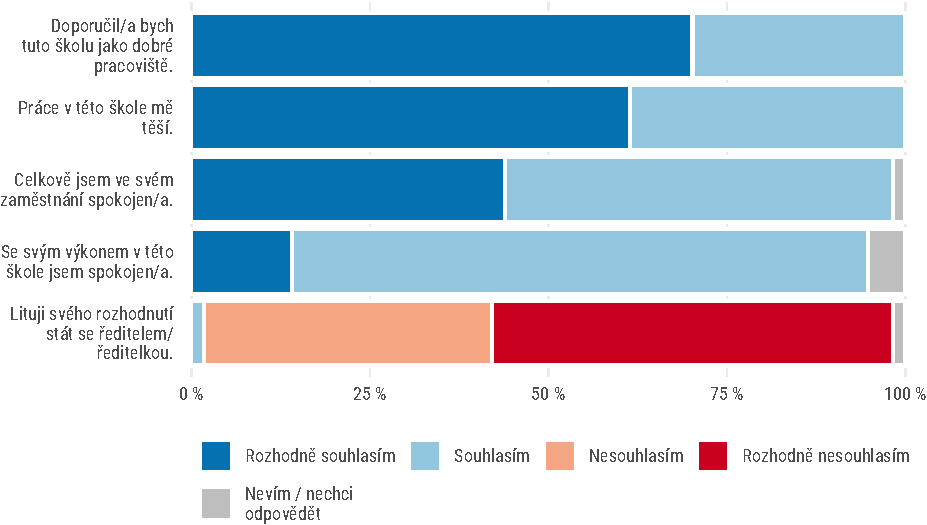
\includegraphics[width=\textwidth]{figs/satisDir-1} 

}

\caption{Postoje k výkonu práce ředitele na dané škole}\label{fig:satisDir}
\end{figure}

Z~dalších otázek týkajících se spokojenosti s~prací si lze povšimnout například toho, že ředitelé jsou spokojeni s~podporou svých zaměstnanců a~mají pocit, že v~jejich školách existuje sdílená vize toho, kam se chtějí posouvat.

\begin{figure}

{\centering 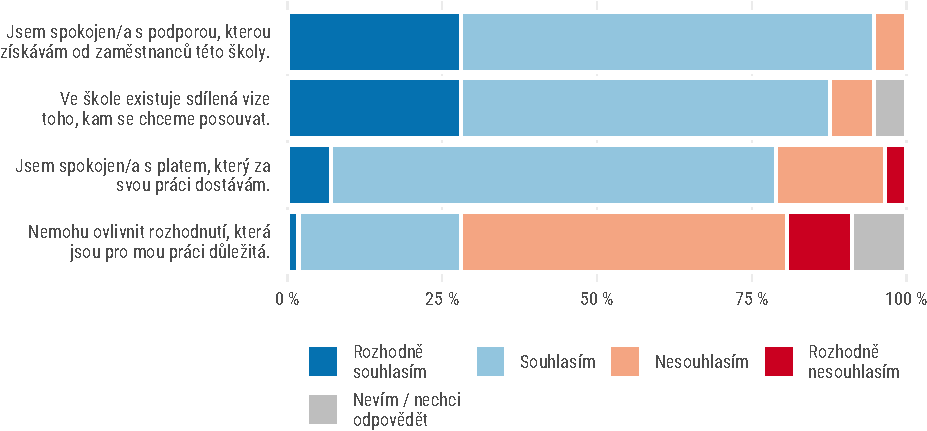
\includegraphics[width=\textwidth]{figs/satisOther-1} 

}

\caption{Další otázky spokojenosti}\label{fig:satisOther}
\end{figure}

\hypertarget{zuxe1kladnuxed-uxfadaje-o-respondentech}{%
\chapter{\texorpdfstring{Základní údaje o~respondentech}{Základní údaje orespondentech}}\label{zuxe1kladnuxed-uxfadaje-o-respondentech}}

Dotazník otevřelo celkem~88 ředitelek a~ředitelů a~67 u~nich ho vyplněný odeslalo. Návratnost tedy činí~71~\%.

\begin{figure}

{\centering 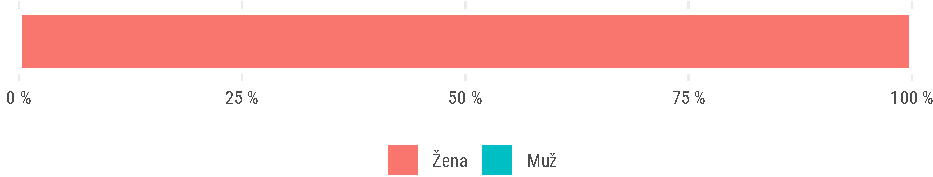
\includegraphics[width=\textwidth]{figs/sex-1} 

}

\caption{Zastoupení pohlaví}\label{fig:sex}
\end{figure}

V~následujícím grafu uvádíme distribuci věku ředitelů, počtu let strávených na pozici ředitele celkem a~také počet let ředitelování na dané škole.

\begin{figure}

{\centering 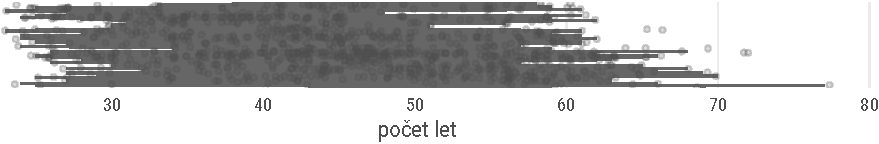
\includegraphics[width=\textwidth]{figs/age-1} 

}

\caption{Věk ředitelů a jejich působení na pozici v této škole / celkově}\label{fig:age}
\end{figure}



\end{document}
